\chapter{Charged pion reconstruction and identification}
\label{ch:reconstruction}
\graphicspath{{Chapter-Reconstruction/figures/}}

Charged particles produced in collisions at the ATLAS \ac{IP} travel helical paths through the \id due to the solenoid magnetic field.
The three subdetectors register hits at various space-point locations as each of these particles passes through them, often 11 silicon and 15--30 \trt hits for a typical particle of sufficiently high \pt.
The trajectories of these particles must be reconstructed from the collection of all the space-point hits in order to infer the initial momentum of all of the collision products.
This procedure is non-trivial and computationally intensive, particularly because the trajectories of charged particles are altered when they pass through detector elements, via ionization energy loss and multiple scattering.

\section{Tracking algorithm}

%% for general track fitting overview see:
%% http://www.phys.ufl.edu/~avery/fitting.html
%% atlas overview see https://cds.cern.ch/record/1435196/files/ATLAS-CONF-2012-042.pdf
%% from \cite{ATLAS:2012jma}

%% discuss seeding before kalman filter?
%% i.e. split into ``pattern finding'' and ``track fitting'', though with NEWT there is ``no clear border'' between these modules
%% discuss inside-out and outside-in separately?

While the classification is not absolute, the ATLAS track reconstruction procedure can be divided roughly into two parts: first track seeds are identified, then tracks are extended and evaluated with a global fit \cite{Cornelissen:2007vba}. %% ATLAS new tracking (NEWT)
Each of these procedures will be described separately in the following sections.
Overall, the reconstruction of collision vertices and the charged-particle products has very good performance, even in the high-luminosity environment of the \lhc with tens of simultaneous collisions along the beamline \cite{ATLAS:2012jma}. %% performance of tracking and vertexing (2012), w/ description of reconstruction

\subsection{Seeding track candidates}

\begin{figure}[t]
  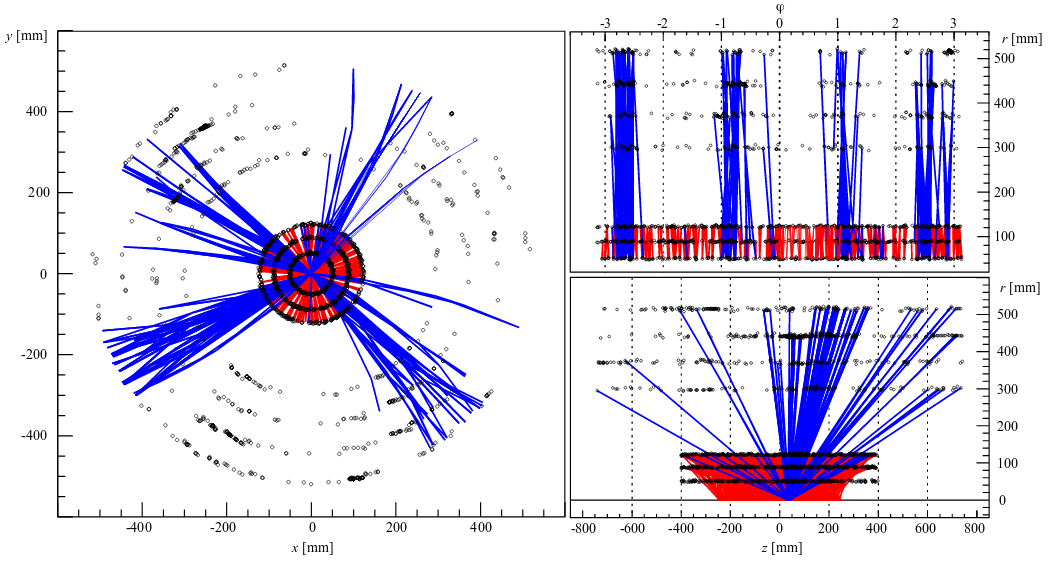
\includegraphics[width=\linewidth]{soft-pub-2007-007_sp_seeds.png}
  \caption{Space-point seeds constructed from two (short, in red) or three (long, in blue) hits in the barrel region of the pixel and \sct. Short seeds are used to determine the $z$-coordinates of predicted vertex positions, which are used to constrain extensions to three or more space points.  (From \Ref{\cite{Cornelissen:2007vba}})}
  \label{fig:trk_seeds}
\end{figure}

The baseline track finding algorithm uses inside-out reconstruction.
Space-points are collected by hits in the silicon detectors by the 3D location of pixel hits and by the crossing point of back-to-back \sct strip pairs with simultaneous hits.
Pairs of space-points from the pixel detector are used to construct short track seeds, which are used to find the longitudinal position of vertices.
A histogram is filled with the $z$-coordinate of straight-line extensions of these track seeds to the beam line and peaks in this distribution are identified with the $z$ position of the vertices.
These $z$-vertices constrain the extension of seeds from two space-points to three (\Cref{fig:trk_seeds}).
The seed search can also be done without the $z$ vertex constraint, inducing a significant increase in computational demands but allows for a greater efficiency to reconstruct decays from certain events.
The seeds with three space-points are fed to the track extension and fitting algorithm.

After the inside-out track reconstruction is completed, an additional round of seeding is performed using an outside-in algorithm called back-tracking.
This process is designed to reconstruct secondary particles, which are generated in the decays of primary particles and so do not necessarily originate from near the beam line.
The \trt drift tube hits do not provide fine-scale information along the straw direction, so seeds are built in the $r - \phi$ plane in the \trt barrel and the $r - z$ plane in the \trt end-cap.
Back-tracking is not well-suited for low-\pt particles, which spiral out of the \id without making it to the \trt, so the targeted particles have reasonably straight-line trajectories.
The Hough transform \cite{Duda:1972:UHT:361237.361242} is used to detect straight-line sets of three \trt hits which are used as track candidate seeds.
The extension of these \trt segments into the silicon detectors are evaluated in multiple $\eta$ slices to accommodate the fact that the seed-finding is done in the transverse plane.

Finally, the remaining silicon hits that have not been used in the inside-out or back-tracking algorithms are used to seed an additional low-\pt track reconstruction.%% ATL-COM-INDET-2012-052 for minbias
Charged particles with $\pt < 400 \MeV$ do not necessarily pass through every layer of the \sct.
These tracks can have a transverse momentum as low as 100 \MeV~ so their transverse radius of curvature is small.
Without a trajectory that is close to a straight line in the transverse plane, a larger set of possible track seeds must be evaluated, so it is only computationally feasible to seed the low-\pt tracking with leftover space-points from the other two tracking algorithms.
The efficiency below $\pt = 400 \MeV$ begins do fall rapidly with decreasing \pt, but a significant fraction of particles in this kinematic region are reconstructed.

\subsection{Track extension and fitting}

\begin{figure}[t]
  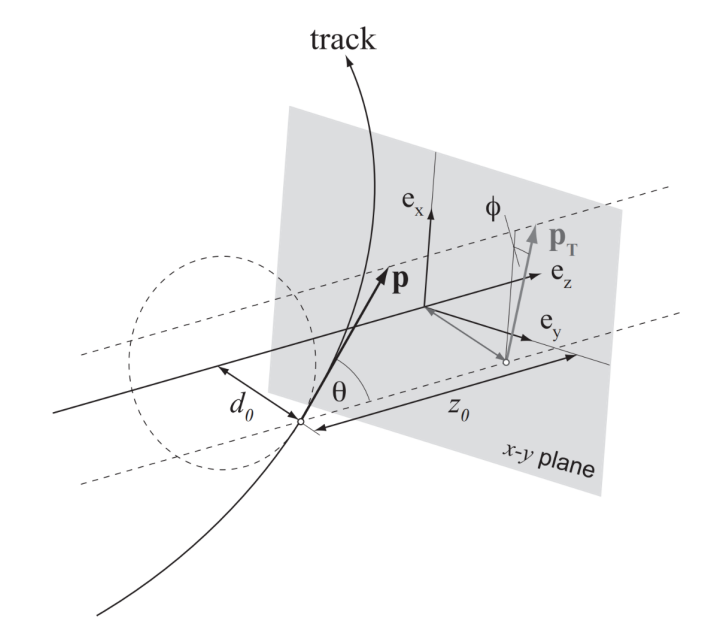
\includegraphics{track_schematic.png}
  \caption{The track parameters defining a helical trajectory.}
  \label{fig:trk_params}
\end{figure}

%% Kalman filter -- dedicated subsection?
A helical track path is defined by the 5-tuple
\( \left( d_0, z_0, \theta, \phi, q/p \right) \)
where $d_0$ and $z_0$ are the transverse and longitudinal distance from the beamspot at the point of closest approach, $\theta$ and $\phi$ are the polar and azimuthal angles of the track at this point, and $q/p$ is the inverse magnitude of the track's total momentum signed by the charge of the particle\footnote{This ratio is related to the transverse radius of curvature $R$ and the axial magnetic field $B$ by $q/p = \sin \theta / B R$.} (\Cref{fig:trk_params}).
However, every interaction with a detector element modifies a charged particle's trajectory through ionization energy loss and multiple scattering.
Since there are tens of hits in most tracks, a typical track has $\mathcal{O}(100)$ parameters in its description, and the parameters before and after a hit are not independent.
It is computationally infeasible to process a single global fit for each track candidate with this many correlated parameters.
A Kalman filter approach is taken instead, which processes a track from one end to the other, updating the parameters and covariance matrix along the way.

The three space-points in a track seed are sufficient to constrain a helical path.
This naive trajectory is used to build a road along which additional silicon hits are checked for.
The Kalman smoother-fitter follows the trajectory and incorporates successive hits into the fit \cite{Cornelissen:2008zza}. %% global chi^2 track fitter
It predicts where hits for a track candidate would be expected in other layers, and a track candidate is penalized if there are no hits near the expected trajectory. %% TODO: more detail on kalman filters?
Under typical LHC circumstances, about 10\% of seeds result in a successful track candidate.

\subsection{Ambiguity solving} %% does this deserve a separate section?

Many of the track candidates at this point have holes, shared hits, or represent fake tracks.
The $\chi^2$ output of the Kalman filter is not a good quantity for determining whether a track is a fake or not\footnote{The $\chi^2$ should follow a corresponding $\chi^2$ distribution, which has a tail that extends to positive infinity. Selecting tracks based on their $\chi^2$ would lead to a biased sample.}.
A track scoring strategy is used that penalizes track candidates for holes using different weights depending on the location of the hole in the detector \cite{Wicke:1998efw}.
In general, measurements from more precise detector systems are given larger weights.
Shared hits from two or more tracks are assigned to the track with the largest score, and the remainder of the tracks with the shared hit are refit neglecting this hit, and their score is re-calculated.
Track candidates with a score that falls below a certain quality threshold are removed, and this process is performed iteratively until the set of tracks remains unchanged.

\subsection{TRT track extension}

The trajectory of each track from the silicon detectors is followed into the \trt, where compatible hits are searched for.
If a possible extension is found, the track is refit and re-scored with the \trt hits.
If the extended track has a higher score than the silicon-only track, then the track is updated with the extension.
Otherwise the original silicon track is kept and the \trt hits are kept as outliers.

\section{Track selection} %% ? does this need its own section? possibly in analysis section

The tracks used for the results in this thesis are inside-out and low-\pt tracks.
Tracks from back-tracking are not used because they are typically secondary particles.
The offline track selection is that used in the \pPb multiplicity analysis \cite{HION-2012-15}, which is based on the \pp \minbias spectra analysis \cite{STDM-2010-06} with some additional cuts on impact parameter ($d_0$ and $z_0$) significance.
\begin{itemize}
\item
  The track must have $\pt \geq 0.1 \GeV$ and $|\eta| < 2.5$.
\item
  A track with $\pt \geq $ 0.1/0.2/0.3 \GeV must have at least 2/4/6 \sct hits.
  These transverse momentum cutoffs correspond approximately to thresholds after which the track is expected to pass through the next \sct layer.
\item
  At least one physical pixel hit is required, and if a B-Layer hit is expected based on the trajectory then there is at least one physical B-Layer hit.
\item
  The transverse and longitudinal impact parameters with respect to the \ac{PV} must satisfy $|d_0^\textrm{PV}| < 1.5 \textrm{ mm}$ and $|z_0^\textrm{PV} \sin\theta| < 1.5 \textrm{ mm}$.
\item
  A significance cut is also placed on the impact parameters such that $|d_0^\textrm{PV}| < 3\sigma_{d_0^\textrm{PV}}$ and $|z_0^\textrm{PV} \sin\theta| < 3\sigma_{z_0^\textrm{PV} \sin\theta}$.
\end{itemize}


\section{Track reconstruction performance}

High-energy \pp and heavy ion collisions are generated with \mc simulations to study the performance of the track reconstruction algorithm.
Proton-lead collision events are generated with \Hijing \cite{Gyulassy:1994ew} and the detector material is simulated with \GEANTFour \cite{Agostinelli:2002hh}.
These simulations are able to provide an accurate description of many track properties, for example the silicon hits per track shown in \Cref{fig:trk_si_hits}.
The efficiency to reconstruct a track in \mc samples is shown in \Cref{fig:trk_eff}.

\begin{figure}[t]
  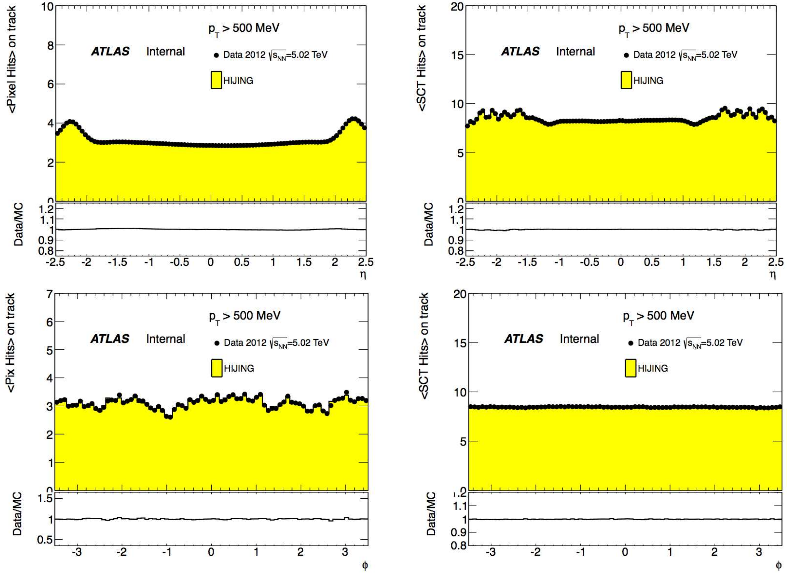
\includegraphics[width=\linewidth]{ATL-COM-PHYS-2013-1017_sihits.png}
  \caption{The mean number of silicon hits on track in Run-1 \pPb collisions as a function of pseudorapidity (top) and azimuthal angle (bottom).}
  \label{fig:trk_si_hits}
\end{figure}

\begin{figure}[t]
  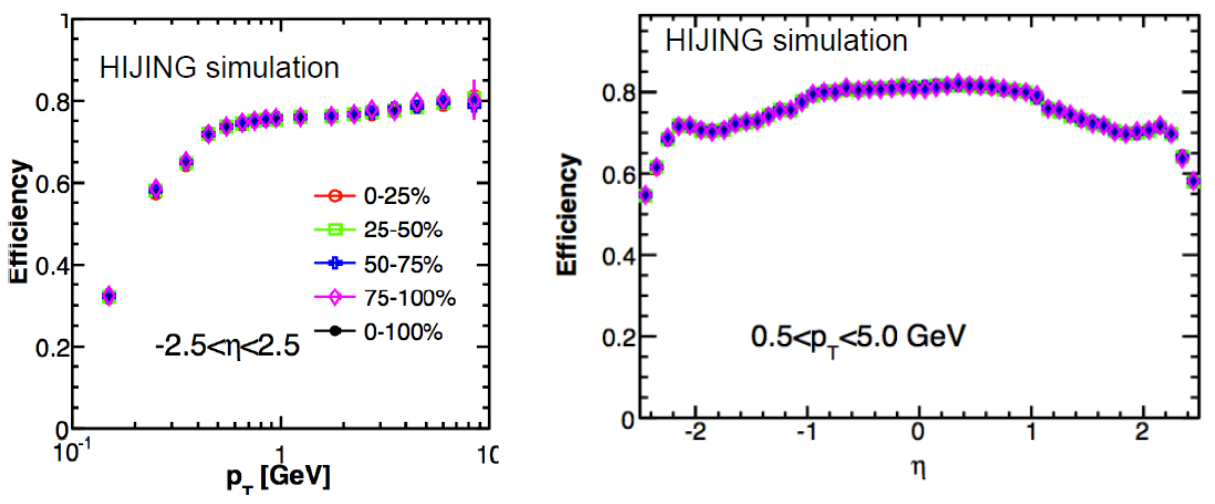
\includegraphics[width=\linewidth]{ATL-COM-PHYS-2013-011_trk_eff.png}
  \caption{The track reconstruction efficiency in Run-1 \pPb collisions as a function of transverse momentum (left) and pseudorapidity (right).}
  \label{fig:trk_eff}
\end{figure}

\section{Pion identification}

\cite{ATLAS-CONF-2011-016}
